\documentclass[a4paper,12pt]{article}

% Компиляция: XeLaTeX (дважды) или pdfLaTeX с установленной кириллицей.
\usepackage{iftex}
\ifPDFTeX
    \usepackage[T2A]{fontenc}
    \usepackage[utf8]{inputenc}
    \usepackage[russian]{babel}
    \usepackage{cmap}
\else
    \usepackage{fontspec}
    \defaultfontfeatures{Ligatures=TeX}
    \setmainfont{NimbusRoman-Regular.otf}[
        BoldFont=NimbusRoman-Bold.otf,
        ItalicFont=NimbusRoman-Italic.otf,
        BoldItalicFont=NimbusRoman-BoldItalic.otf]
    \setsansfont{NimbusSans-Regular.otf}[
        BoldFont=NimbusSans-Bold.otf,
        ItalicFont=NimbusSans-Italic.otf,
        BoldItalicFont=NimbusSans-BoldItalic.otf]
    \setmonofont{DejaVu Sans Mono}[Scale=0.85]
    \newfontfamily\cyrillicfont{NimbusRoman-Regular.otf}[
        Script=Default,BoldFont=NimbusRoman-Bold.otf,
        ItalicFont=NimbusRoman-Italic.otf,
        BoldItalicFont=NimbusRoman-BoldItalic.otf]
    \newfontfamily\cyrillicfontsf{NimbusSans-Regular.otf}[
        Script=Default,BoldFont=NimbusSans-Bold.otf,
        ItalicFont=NimbusSans-Italic.otf,
        BoldItalicFont=NimbusSans-BoldItalic.otf]
    \newfontfamily\cyrillicfonttt{DejaVu Sans Mono}[Script=Default,Scale=0.85]
    \usepackage{polyglossia}
    \setdefaultlanguage{russian}
\fi

\usepackage{amsmath}
\usepackage{amssymb}
\usepackage{amsfonts}
\usepackage{graphicx}
\usepackage{geometry}
\usepackage{listings}
\usepackage{xcolor}
\usepackage{hyperref}
\usepackage{float}
\usepackage{booktabs}
\usepackage{tabularx}
\usepackage{array}
\usepackage{caption}
\usepackage{enumitem}
\usepackage{needspace}
\usepackage{microtype}

\geometry{left=2cm, right=1.5cm, top=2cm, bottom=2cm}
\setlength{\parindent}{1.25cm}
\setlength{\parskip}{0pt}
\setlength{\emergencystretch}{6em}
\setlist[itemize]{topsep=4pt,itemsep=2pt,parsep=0pt}
\setlist[enumerate]{topsep=4pt,itemsep=2pt,parsep=0pt}
\captionsetup{font=small,labelsep=period,justification=centering}
\hypersetup{unicode=true,colorlinks=true,linkcolor=black,urlcolor=blue,
    pdftitle={Лабораторная работа №1. Линейная и логистическая регрессия},
    pdfauthor={Михайлов Петр Сергеевич}}
\graphicspath{{figures/}}
\newcommand{\code}[1]{\texttt{#1}}
\newcommand{\R}{\mathbb{R}}

\lstdefinestyle{mypython}{
    language=Python,
    basicstyle=\ttfamily\scriptsize,
    keywordstyle=\color{blue}\bfseries,
    stringstyle=\color{red},
    commentstyle=\color{green!60!black},
    numbers=left,
    numberstyle=\tiny\color{gray},
    stepnumber=1,
    numbersep=8pt,
    showspaces=false,
    showstringspaces=false,
    tabsize=4,
    frame=single,
    rulecolor=\color{black},
    breaklines=true,
    breakatwhitespace=false,
    captionpos=b,
    xleftmargin=15pt,
    xrightmargin=5pt,
    framexleftmargin=12pt,
    backgroundcolor=\color{gray!5}
}
\lstset{style=mypython}

\begin{document}

% ===========================================================================
% ТИТУЛЬНЫЙ ЛИСТ
% ===========================================================================
\begin{titlepage}
    \centering

    {\fontsize{11}{13}\selectfont
    \textbf{Министерство науки и высшего образования Российской Федерации}\par}
    \vspace{0.12cm}

    {\fontsize{7}{10}\selectfont
    ФЕДЕРАЛЬНОЕ ГОСУДАРСТВЕННОЕ АВТОНОМНОЕ ОБРАЗОВАТЕЛЬНОЕ УЧРЕЖДЕНИЕ ВЫСШЕГО ОБРАЗОВАНИЯ\par}

    \vspace{0.2cm}

    {\fontsize{14}{17}\selectfont
    \textbf{«НАЦИОНАЛЬНЫЙ ИССЛЕДОВАТЕЛЬСКИЙ УНИВЕРСИТЕТ ИТМО»}\par}

    \vspace{1cm}

    {\fontsize{12}{14}\selectfont
    \textbf{Факультет программной инженерии и компьютерной техники}\par}

    \vspace{1cm}

    {\fontsize{12}{14}\selectfont
    \textbf{Дисциплина: Системы искусственного интеллекта}\par}

    \vspace*{\fill}

    {\fontsize{18}{22}\selectfont
    \textbf{ЛАБОРАТОРНАЯ РАБОТА №1}\par}

    \vspace{0.5cm}

    {\fontsize{14}{17}\selectfont
    \textbf{по теме: «Линейная и логистическая регрессия»}\par}

    \vspace{2cm}

    \begin{flushright}
        \fontsize{12}{14}\selectfont
        Выполнил:\par
        Михайлов Петр Сергеевич\par
        Группа: P3311\par

        \vspace{1em}

        Преподаватель:\par
        Королёва Юлия Александровна
    \end{flushright}

    \vfill

    {\fontsize{12}{14}\selectfont Санкт-Петербург, 2026\par}
\end{titlepage}

\setcounter{page}{2}
\tableofcontents
\newpage

% ===========================================================================
\section{Цель и задачи работы}

\textbf{Цель лабораторной работы} --- самостоятельно реализовать линейную
и логистическую регрессии с обучением градиентным спуском, подготовить
данные для регрессии и бинарной классификации и оценить качество моделей
в сравнении с простыми базовыми решениями.

Задачи работы:
\begin{enumerate}
    \item Исследовать наборы Bike Sharing Dataset и Spaceship Titanic,
    выделить входные признаки $X$ и целевую переменную $y$.
    \item Самостоятельно реализовать разбиение данных, заполнение пропусков,
    стандартизацию и one-hot кодирование без готовых ML-компонентов.
    \item Реализовать классы \code{LinearRegression} и
    \code{LogisticRegression}, ручной расчёт градиентов и обновление параметров.
    \item Сохранить историю функции потерь и построить графики обучения.
    \item Выбрать настройки по валидационной выборке, вычислить требуемые
    метрики на тестовой выборке и сравнить их с baseline.
    \item Проверить собственные метрики с помощью \code{sklearn.metrics}
    и сформулировать выводы.
\end{enumerate}

Основной воспроизводимый эксперимент и программный отчёт находятся
в \code{lab1.ipynb}. Дополнительная отправка прогнозов на Kaggle
описана в разделе~\ref{sec:kaggle}.
Код и ноутбук размещаются в \href{https://github.com/Axe-On-You/Artificial-intelligence-systems/tree/main/\%D0\%9B\%D0\%B0\%D0\%B1\%D0\%BE\%D1\%80\%D0\%B0\%D1\%82\%D0\%BE\%D1\%80\%D0\%BD\%D0\%B0\%D1\%8F\%201}{папке лабораторной на GitHub}.

\section{Используемые методы}

\subsection{Линейная регрессия}

Для $N$ объектов с $D$ подготовленными признаками используются матрица
$X\in\R^{N\times D}$, вектор ответов $y\in\R^N$, вектор весов
$w\in\R^D$ и свободный член $b\in\R$. Предсказание модели:
\begin{equation}
    \hat y=Xw+b.
\end{equation}
Свободный член прибавляется ко всем компонентам вектора предсказаний.
Минимизируется средняя квадратичная ошибка:
\begin{equation}
    L_{\mathrm{MSE}}=\frac{1}{N}\sum_{i=1}^{N}(\hat y_i-y_i)^2.
\end{equation}
Обозначив $e=\hat y-y$, получим градиенты:
\begin{equation}
    \nabla_w L_{\mathrm{MSE}}=\frac{2}{N}X^\top e,
    \qquad
    \frac{\partial L_{\mathrm{MSE}}}{\partial b}
    =\frac{2}{N}\sum_{i=1}^{N} e_i.
\end{equation}

\subsection{Логистическая регрессия}

Для бинарной классификации вычисляются линейная оценка $z$ и вероятность
положительного класса $p$:
\begin{equation}
    z=Xw+b,\qquad p=\sigma(z),\qquad
    \sigma(z)=\frac{1}{1+\exp(-z)}.
\end{equation}
Для $y_i\in\{0,1\}$ используется бинарная кросс-энтропия:
\begin{equation}
    L_{\mathrm{BCE}}
    =-\frac{1}{N}\sum_{i=1}^{N}
    \bigl[y_i\ln p_i+(1-y_i)\ln(1-p_i)\bigr].
\end{equation}
В реализации значение потерь рассчитывается по эквивалентной устойчивой
формуле, не требующей прямого логарифмирования вероятностей:
\begin{equation}
    L_{\mathrm{BCE}}
    =\frac{1}{N}\sum_{i=1}^{N}
    \left[\max(z_i,0)-y_i z_i+
    \ln\bigl(1+\exp(-|z_i|)\bigr)\right].
\end{equation}
Градиенты имеют вид:
\begin{equation}
    \nabla_w L_{\mathrm{BCE}}=\frac{1}{N}X^\top(p-y),
    \qquad
    \frac{\partial L_{\mathrm{BCE}}}{\partial b}
    =\frac{1}{N}\sum_{i=1}^{N}(p_i-y_i).
\end{equation}
Метод \code{predict\_proba} возвращает вектор вероятностей класса~1,
а \code{predict} применяет фиксированный порог $t=0.5$:
$\hat y_i=1$ при $p_i\geq t$ и $\hat y_i=0$ в остальных случаях.

\subsection{Обучение и протокол оценки}

Обе модели обучаются полным градиентным спуском:
\begin{equation}
    w\leftarrow w-\alpha\nabla_w L,
    \qquad b\leftarrow b-\alpha\frac{\partial L}{\partial b}.
\end{equation}
Каждый шаг использует всю обучающую выборку, поэтому одна эпоха соответствует
одному обновлению параметров. Начальные веса и свободный член равны нулю.
Значение loss сохраняется \emph{после} обновления в \code{history\_}.

Данные разделяются примерно в отношении 60/20/20 на train, validation и test.
Для первого разбиения используется seed~42, для выделения validation
из оставшейся части --- seed~43. Разбиения реализованы самостоятельно
по индексам строк; проверено отсутствие пересечений и потерь строк.

Параметры предобработки и веса модели определяются только по train.
Validation используется для выбора learning rate и числа эпох.
После выбора настроек исходная модель не переобучается на объединённых
частях, а test используется для итогового сравнения с baseline.
Такой порядок предотвращает влияние тестовых данных на настройку модели.

% ===========================================================================
\section{Часть A. Линейная регрессия}

\subsection{Исследование данных и выбор признаков}

Используется файл \code{day.csv} набора Bike Sharing Dataset:
731 строка и 16 столбцов, период с 1 января 2011 года по 31 декабря 2012 года.
Один объект соответствует одному дню; целевая переменная
$y=\code{cnt}$ --- число аренд за день. Пропуски и полностью
повторяющиеся строки отсутствуют. Значения \code{cnt} лежат в диапазоне
от 22 до 8714, среднее по исходному набору составляет около 4504.35.

Из $X$ исключены \code{casual} и \code{registered}, поскольку для всех строк
выполняется \code{cnt = casual + registered}. Их использование означало бы
утечку целевого ответа. Также исключены идентификатор \code{instant}
и исходная дата \code{dteday}; календарная информация представлена
отдельными признаками.

\begin{figure}[H]
    \centering
    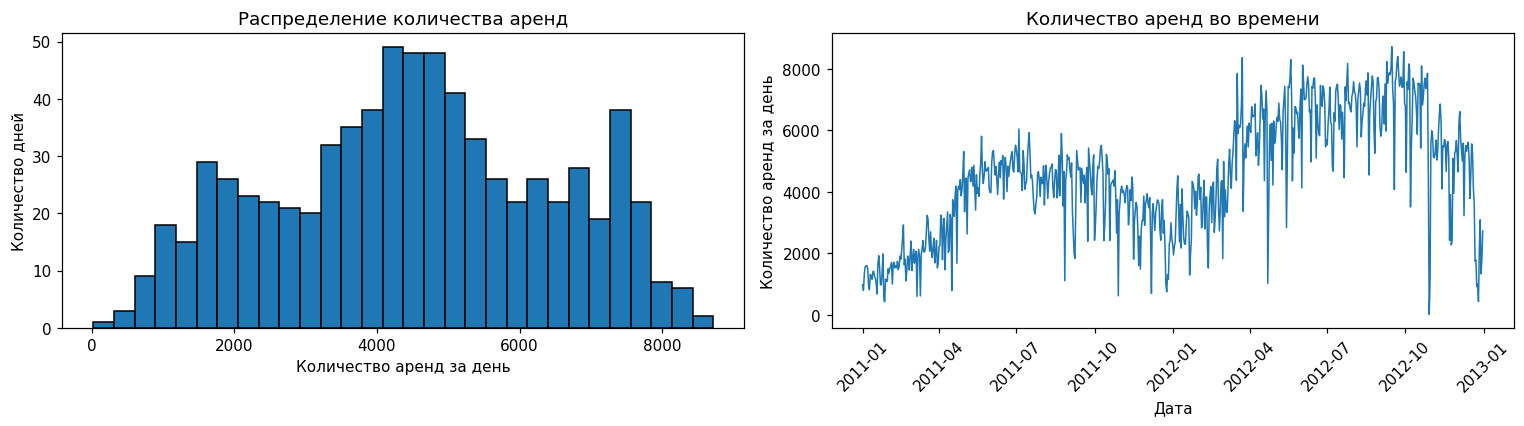
\includegraphics[width=\linewidth]{bike_overview.png}
    \caption{Распределение целевой переменной и изменение количества аренд во времени.}
    \label{fig:bike-overview}
\end{figure}

\subsection{Предобработка и разбиение}

Оставшиеся 11 входных столбцов разделены на три группы:
\begin{itemize}
    \item числовые: \code{temp}, \code{atemp}, \code{hum}, \code{windspeed};
    \item бинарные: \code{yr}, \code{holiday}, \code{workingday};
    \item категориальные: \code{season}, \code{mnth}, \code{weekday},
    \code{weathersit}.
\end{itemize}

Для каждого числового признака выполняется стандартизация
$x'=(x-\mu_{\mathrm{train}})/s_{\mathrm{train}}$.
Стандартное отклонение вычисляется с \code{ddof=0};
для постоянного столбца масштаб заменяется единицей.
Бинарные признаки сохраняются без изменений.

Категории определяются по train и кодируются собственным one-hot
преобразованием. Число индикаторов равно $4+12+7+3=26$.
Вместе с четырьмя числовыми и тремя бинарными признаками получается
$D=33$. Неизвестная категория в этой реализации кодируется нулями
соответствующего блока. Целевая переменная не масштабируется.

\begin{table}[H]
    \centering
    \caption{Размеры выборок Bike Sharing после подготовки признаков.}
    \begin{tabular}{lrr}
        \toprule
        Выборка & Размер $X$ & Размер $y$\\
        \midrule
        Train & $438\times33$ & $438$\\
        Validation & $146\times33$ & $146$\\
        Test & $147\times33$ & $147$\\
        \bottomrule
    \end{tabular}
\end{table}

После преобразования проверены согласованность размерностей и отсутствие
NaN и бесконечных значений. На train средние стандартизированных числовых
признаков близки к нулю, стандартные отклонения равны единице.

\subsection{Выбор настроек и обучение}

Сравниваются девять комбинаций:
$\alpha\in\{0.005,0.01,0.05\}$ и
число эпох $\in\{1000,3000,5000\}$.
Каждая модель обучается на train; критерий выбора ---
минимальный RMSE на validation.

\begin{table}[H]
    \centering
    \caption{Подбор настроек линейной регрессии.}
    \begin{tabular}{rrrr}
        \toprule
        Learning rate & Эпохи & Train RMSE & Validation RMSE\\
        \midrule
        0.005 & 1000 & 802.4534 & 770.0379\\
        0.005 & 3000 & 780.1029 & 760.7358\\
        0.005 & 5000 & 777.0977 & 762.8595\\
        \textbf{0.010} & \textbf{1000} & \textbf{784.9002} & \textbf{759.8197}\\
        0.010 & 3000 & 776.4915 & 763.5563\\
        0.010 & 5000 & 775.5239 & 765.5704\\
        0.050 & 1000 & 775.5232 & 765.5725\\
        0.050 & 3000 & 775.0284 & 769.6367\\
        0.050 & 5000 & 775.0182 & 770.2764\\
        \bottomrule
    \end{tabular}
    \label{tab:linear-search}
\end{table}

Выбраны $\alpha=0.01$ и 1000 эпох. При увеличении числа эпох train RMSE
продолжает уменьшаться, но validation RMSE не улучшается.
Следовательно, минимальная ошибка обучения сама по себе не определяет
лучшую настройку для новых объектов.

\begin{figure}[H]
    \centering
    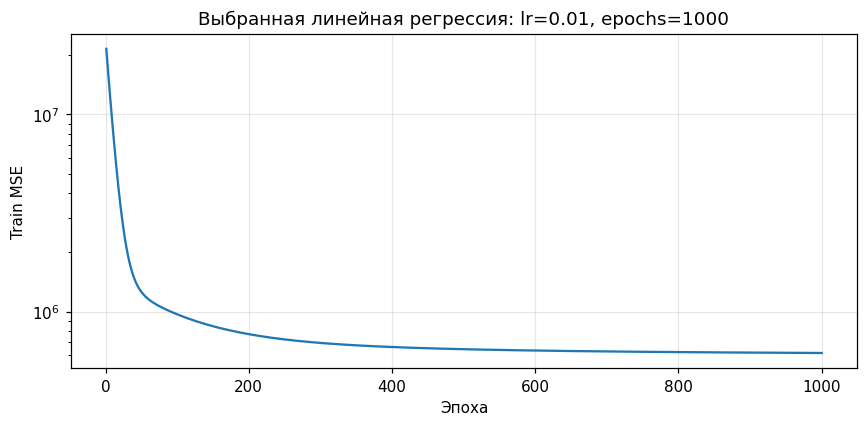
\includegraphics[width=0.88\linewidth]{bike_loss.png}
    \caption{История MSE выбранной линейной регрессии: $\alpha=0.01$, 1000 эпох.}
    \label{fig:bike-loss}
\end{figure}

\subsection{Итоговые метрики и сравнение с baseline}

Для оценки используются:
\begin{align}
    \mathrm{MAE} &= \frac{1}{N}\sum_i |y_i-\hat y_i|,\\
    \mathrm{RMSE} &= \sqrt{\frac{1}{N}\sum_i(y_i-\hat y_i)^2},\\
    R^2 &=1-\frac{\sum_i(y_i-\hat y_i)^2}
    {\sum_i(y_i-\bar y)^2}.
\end{align}
Здесь $N$ и $\bar y$ относятся к оцениваемой выборке.
При оценке test это 147 дней и среднее их реальных значений \code{cnt}.
MAE и RMSE измеряются в числе аренд; большие промахи сильнее влияют на RMSE.

Mean baseline каждому объекту предсказывает среднее \code{cnt}
по \emph{train}, равное примерно 4487.84.
Среднее test не используется для построения baseline.

\begin{table}[H]
    \centering
    \caption{Качество регрессии на test, 147 дней.}
    \begin{tabular}{lrrr}
        \toprule
        Модель & MAE & RMSE & $R^2$\\
        \midrule
        Mean baseline & 1511.9331 & 1823.2899 & $-0.0011$\\
        Linear Regression & \textbf{555.9205} & \textbf{723.3595} & \textbf{0.8424}\\
        \bottomrule
    \end{tabular}
    \label{tab:linear-test}
\end{table}

Линейная регрессия уменьшает MAE примерно на 63.2\%, RMSE --- на 60.3\%
относительно baseline. Значение $R^2=0.8424$ означает уменьшение суммы
квадратов ошибок примерно на 84.24\% относительно постоянного прогноза
среднего \emph{test}; это не доля точно предсказанных дней.

\begin{figure}[H]
    \centering
    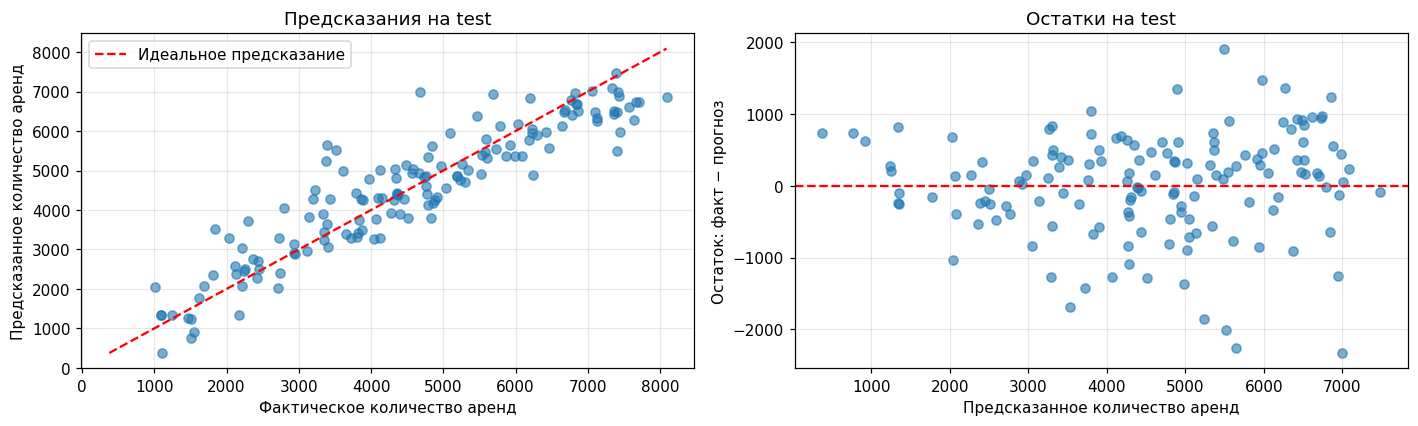
\includegraphics[width=\linewidth]{bike_predictions.png}
    \caption{Прогнозы выбранной модели и остатки $r=y-\hat y$ на test.}
    \label{fig:bike-predictions}
\end{figure}

Модель воспроизводит общую зависимость количества аренд от признаков,
однако отдельные крупные ошибки сохраняются. Случайный split оценивает
отложенные дни исходного периода и не является проверкой прогноза
будущего временного интервала.

% ===========================================================================
\section{Часть B. Логистическая регрессия}

\subsection{Исследование данных}

Используется размеченный файл \code{train.csv}:
8693 строки и 14 столбцов. Один объект --- пассажир.
Целевая переменная \code{Transported} преобразуется в классы:
\code{False} $=0$, \code{True} $=1$.
Положительный класс означает перемещение пассажира в другое измерение.

В наборе 4315 объектов класса~0 (49.64\%) и 4378 объектов класса~1
(50.36\%). Полностью совпадающие строки и повторяющиеся
\code{PassengerId} отсутствуют. В большинстве входных столбцов есть
пропуски; их доля составляет примерно 2.1--2.5\%.
Например, в \code{Age} отсутствуют 179 значений, в \code{CryoSleep} --- 217.

Из входных признаков исключены \code{PassengerId} и \code{Name}.
Соревновательный \code{test.csv} не участвует в основном локальном
эксперименте: train, validation и test формируются из размеченного
\code{train.csv}.

\subsection{Предобработка и стратификация}

Выполнено собственное стратифицированное разбиение, сохраняющее
приблизительно одинаковые доли классов:
\begin{table}[H]
    \centering
    \caption{Выборки Spaceship Titanic после предобработки.}
    \begin{tabular}{lrrrr}
        \toprule
        Выборка & Объекты & Класс 0 & Класс 1 & Признаки\\
        \midrule
        Train & 5215 & 2589 & 2626 & 33\\
        Validation & 1739 & 863 & 876 & 33\\
        Test & 1739 & 863 & 876 & 33\\
        \bottomrule
    \end{tabular}
\end{table}

Предобработка выполняется в следующем порядке:
\begin{enumerate}
    \item \code{Cabin} вида \code{B/0/P} разделяется на палубу
    \code{CabinDeck}, номер \code{CabinNumber} и сторону \code{CabinSide}.
    \item Числовые пропуски заполняются медианами train.
    Медиана возраста равна 27, номера каюты --- 419,
    каждого из пяти признаков расходов --- 0.
    \item К расходам \code{RoomService}, \code{FoodCourt},
    \code{ShoppingMall}, \code{Spa}, \code{VRDeck}
    применяется преобразование $x\mapsto\ln(1+x)$.
    \item Семь числовых признаков стандартизируются по train.
    \item Шесть категориальных признаков кодируются one-hot.
    Для пропусков и новых категорий используется \code{Unknown}.
\end{enumerate}

Категориальные признаки: \code{HomePlanet}, \code{Destination},
\code{CryoSleep}, \code{VIP}, \code{CabinDeck}, \code{CabinSide}.
После преобразования получается 7 числовых и 26 индикаторных столбцов,
всего 33 признака. Строки с пропусками не удаляются.
Медианы, параметры масштабирования и словари категорий обучаются
только на train; на validation и test вызывается только \code{transform}.

\subsection{Выбор настроек и обучение}

Сравниваются четыре комбинации параметров.
Критерий выбора --- минимальный LogLoss на validation.
Порог классификации во всех экспериментах равен 0.5.

\begin{table}[H]
    \centering
    \caption{Подбор настроек логистической регрессии.}
    \small
    \begin{tabular}{rrrrr}
        \toprule
        Learning rate & Эпохи & Train BCE & Val LogLoss & Val Accuracy\\
        \midrule
        0.01 & 1000 & 0.501210 & 0.502987 & 0.767683\\
        0.05 & 1000 & 0.478882 & 0.481633 & 0.767108\\
        0.05 & 3000 & 0.476891 & 0.480083 & 0.767108\\
        \textbf{0.10} & \textbf{3000} & \textbf{0.476508} & \textbf{0.479952} & \textbf{0.768833}\\
        \bottomrule
    \end{tabular}
    \label{tab:logistic-search}
\end{table}

Выбраны $\alpha=0.1$ и 3000 эпох.
История потерь выбранной модели приведена
на рисунке~\ref{fig:logistic-loss}.

\begin{figure}[H]
    \centering
    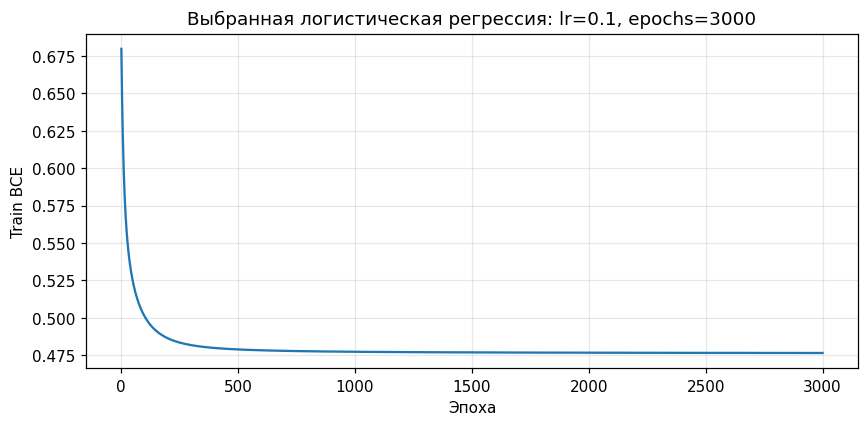
\includegraphics[width=0.88\linewidth]{logistic_loss.png}
    \caption{История BCE выбранной логистической регрессии:
    $\alpha=0.1$, 3000 эпох.}
    \label{fig:logistic-loss}
\end{figure}

\subsection{Метрики, baseline и матрица ошибок}

Рассчитываются Accuracy, Precision, Recall, F1 и LogLoss.
Для положительного класса~1:
\begin{align}
    \mathrm{Accuracy}&=\frac{TP+TN}{TP+TN+FP+FN},\\
    \mathrm{Precision}&=\frac{TP}{TP+FP},\qquad
    \mathrm{Recall}=\frac{TP}{TP+FN},\\
    F_1&=\frac{2TP}{2TP+FP+FN}.
\end{align}
LogLoss вычисляется по формуле BCE на тестовых вероятностях.
Перед логарифмированием вероятности ограничиваются интервалом
$[10^{-15},1-10^{-15}]$.

Majority baseline всем объектам предсказывает класс~1 ---
наиболее частый класс train. Для расчёта его LogLoss используется
постоянная вероятность, равная доле класса~1 в train:
$p_{\mathrm{base}}\approx0.503547$.

\begin{table}[H]
    \centering
    \caption{Качество классификации на test, 1739 пассажиров.}
    \small
    \begin{tabular}{lrrrrr}
        \toprule
        Модель & Accuracy & Precision & Recall & F1 & LogLoss\\
        \midrule
        Majority baseline & 0.503738 & 0.503738 & 1.000000 & 0.669981 & 0.693119\\
        Logistic Regression & 0.776883 & 0.768132 & 0.797945 & 0.782755 & 0.478761\\
        \bottomrule
    \end{tabular}
    \label{tab:logistic-test}
\end{table}

Логистическая регрессия правильно классифицировала
$1351$ из $1739$ пассажиров:
$TN=652$, $FP=211$, $FN=177$, $TP=699$.
Строки матрицы ошибок соответствуют истинным классам,
столбцы --- предсказанным.

\begin{figure}[H]
    \centering
    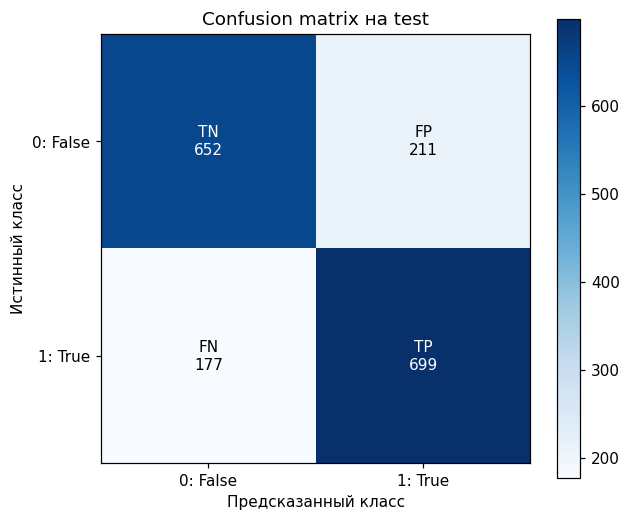
\includegraphics[width=0.55\linewidth]{confusion_matrix.png}
    \caption{Матрица ошибок выбранной логистической регрессии на test.}
    \label{fig:confusion}
\end{figure}

Прирост Accuracy относительно baseline составляет 27.31 процентного
пункта; LogLoss снижается с 0.693119 до 0.478761.
Recall baseline равен единице, потому что он относит всех пассажиров
к положительному классу. При этом возникают 863 ложных положительных
ответа. Это показывает, почему одной метрики недостаточно.

Значения train BCE, validation LogLoss и test LogLoss близки:
0.476508, 0.479952 и 0.478761 соответственно.
В рамках проведённого разбиения выраженного разрыва между
обучением и отложенными данными не наблюдается.

% ===========================================================================
\section{Реализация и проверка результатов}

\subsection{Структура проекта}

\begin{table}[H]
    \centering
    \caption{Основные файлы лабораторной работы.}
    \small
    \begin{tabularx}{\linewidth}{@{}lX@{}}
        \toprule
        Файл & Назначение\\
        \midrule
        \code{lab1.ipynb} & Исследование данных, эксперименты, графики и выводы.\\
        \code{models/linear\_regression.py} & Линейная модель, MSE и градиентный спуск.\\
        \code{models/logistic\_regression.py} & Логистическая модель, sigmoid и устойчивая BCE.\\
        \code{preprocessing.py} & Подготовка признаков обоих наборов данных.\\
        \code{split.py} & Обычное и стратифицированное разбиения по индексам.\\
        \code{evaluation.py} & Собственные метрики регрессии и классификации.\\
        \code{make\_submission.py} & Дополнительное обучение и подготовка CSV для Kaggle.\\
        \bottomrule
    \end{tabularx}
\end{table}

PyTorch используется для тензоров типа \code{float64} и матричных
вычислений на CPU. Готовые модели, слои \code{torch.nn},
оптимизаторы \code{torch.optim} и автоматическое дифференцирование
не используются. Pandas применяется для чтения и обработки таблиц,
NumPy --- для работы с массивами, split, предобработки и метрик,
Matplotlib --- для визуализации.

\Needspace{10\baselineskip}
Ключевой шаг линейной регрессии:
\begin{lstlisting}
predictions = x_tensor @ self.weights_ + self.bias_
errors = predictions - y_tensor
dw = (2.0 / n_samples) * (x_tensor.T @ errors)
db = 2.0 * errors.mean()
self.weights_ -= self.learning_rate * dw
self.bias_ -= self.learning_rate * db
\end{lstlisting}

\Needspace{11\baselineskip}
Ключевой шаг логистической регрессии:
\begin{lstlisting}
logits = x_tensor @ self.weights_ + self.bias_
probabilities = torch.sigmoid(logits)
errors = probabilities - y_tensor
dw = (x_tensor.T @ errors) / n_samples
db = errors.mean()
self.weights_ -= self.learning_rate * dw
self.bias_ -= self.learning_rate * db
\end{lstlisting}

Оба класса имеют методы \code{\_\_init\_\_}, \code{fit}, \code{predict};
логистическая модель дополнительно имеет \code{predict\_proba}.
В \code{fit} проверяются входные данные, выполняется обучение с нуля
и сохраняется история loss. Методы прогнозирования не изменяют параметры
и проверяют факт обучения и число признаков.

\subsection{Проверка и воспроизводимость}

В ноутбуке проверяются непересечение частей, полнота распределения строк,
совпадение числа признаков и отсутствие NaN и бесконечных значений
после предобработки. Для воспроизведения основного эксперимента
необходимо установить зависимости из \code{requirements.txt},
открыть \code{lab1.ipynb} из корня проекта и выполнить все ячейки
в чистом ядре по порядку.

В последней ячейке значения собственных метрик сравниваются
с \code{sklearn.metrics} на одинаковых ответах и прогнозах.
Для чисел используется \code{assert\_allclose}
с \code{rtol=1e-10}, \code{atol=1e-12};
для confusion matrix --- точное сравнение массивов.
Все проверки пройдены. Различие LogLoss составляет около
$5.55\cdot10^{-17}$, остальные выведенные значения совпадают.

Данная проверка подтверждает согласованность вычисления метрик
с эталонными функциями, но сама по себе не доказывает корректность
всей модели или отсутствие утечек. Отсутствие утечек обеспечивается
отдельно порядком split, fit и transform.

\subsection{Ограничения и возможные улучшения}

Случайное разбиение Bike Sharing не оценивает качество на будущем периоде.
В Spaceship Titanic разделяются отдельные пассажиры, поэтому участники
одной группы могут оказаться в разных частях. Для проверки переноса
на новые группы необходимо отдельное групповое разбиение.

Текущая линейная модель не содержит квадрата температуры и явных
взаимодействий признаков. Полное one-hot кодирование вместе с bias
создаёт линейно зависимые столбцы; предсказания можно обучать
градиентным спуском, но отдельные коэффициенты могут быть неединственными.
Также близки по смыслу признаки \code{temp} и \code{atemp}.

Возможные направления развития: хронологический и групповой split,
проверка нелинейных признаков, регуляризация и остановка по validation.
Это предложения для последующих экспериментов, а не реализованные
функции текущих моделей.

% ===========================================================================
\section{Дополнительный эксперимент: отправка на Kaggle}
\label{sec:kaggle}

После завершения локального эксперимента подготовлен отдельный файл
\code{make\_submission.py}. Существующие модели, предобработка и ноутбук
для этого не изменялись.

Для конкурсного прогноза создан новый предобработчик и новый экземпляр
логистической модели. Они обучены на всех 8693 размеченных строках
\code{train.csv}. Применены ранее выбранные настройки:
$\alpha=0.1$, 3000 эпох, порог 0.5.
Конкурсный \code{test.csv} из 4277 строк используется только
для преобразования сохранённым предобработчиком и получения прогнозов.

Получен файл \code{submission.csv} с двумя столбцами:
\code{PassengerId} и \code{Transported}. Идентификаторы сохранены
в исходном порядке, прогнозы записаны как \code{True}/\code{False},
дополнительный индекс не записан.
Получено 2044 прогноза \code{False} и 2233 прогноза \code{True}.
Итоговая BCE на полном обучающем наборе равна 0.476576.

Отправка успешно принята Kaggle. Отображённая оценка Accuracy:
\begin{equation}
    \mathrm{Accuracy}_{\mathrm{Kaggle}}=0.78045
    \quad (78.045\%).
\end{equation}
Она близка к локальной test Accuracy $0.776883$;
разница составляет около 0.357 процентного пункта.
Оценки получены на разных объектах и для моделей, обученных
на разном количестве данных, поэтому это не контролируемое сравнение
влияния размера train.

Это дополнительная внешняя проверка.
Он не заменяет основной локальный эксперимент и не использовался
для выбора его гиперпараметров.

% ===========================================================================
\section{Выводы}

В ходе лабораторной работы самостоятельно реализованы линейная
и логистическая регрессии с полным градиентным спуском.
Расчёт градиентов и обновление параметров выполнены вручную
по формулам изученных методов; PyTorch использован как средство
тензорных вычислений. Самостоятельно реализованы split,
предобработка и требуемые метрики.

Для Bike Sharing после удаления признаков, раскрывающих целевую
переменную, и подготовки 33 признаков получены
MAE $=555.9205$, RMSE $=723.3595$, $R^2=0.8424$.
Линейная модель существенно превосходит прогноз среднего train.

Для Spaceship Titanic выполнены обработка пропусков, выделение
признаков каюты, логарифмирование расходов, стандартизация
и one-hot кодирование. Логистическая модель получила
Accuracy $=0.776883$, F1 $=0.782755$, LogLoss $=0.478761$,
превысив majority baseline по Accuracy на 27.31 процентного пункта.
Дополнительная отправка на Kaggle дала Accuracy $=0.78045$.

Истории потерь и графики подтверждают снижение обучающего loss
при выбранных настройках. Сравнение конфигураций показывает,
что дополнительные эпохи не обязательно улучшают качество
на отложенных объектах. Разделение train/validation/test
позволило выбирать настройки без использования итогового test.
Собственные метрики согласуются со \code{sklearn.metrics}.

\clearpage
\begin{thebibliography}{9}
\addcontentsline{toc}{section}{Список использованных материалов}
    \bibitem{lecture}
    Вводная презентация по дисциплине «Системы искусственного интеллекта».
    Учебные материалы курса, 2026.
    \bibitem{task}
    Лабораторная работа №1: Linear Regression и Logistic Regression.
    Техническое задание.
    \bibitem{bike}
    Bike Sharing Dataset. Kaggle.
    \url{https://www.kaggle.com/datasets/marklvl/bike-sharing-dataset}.
    \bibitem{spaceship}
    Spaceship Titanic. Kaggle.
    \url{https://www.kaggle.com/competitions/spaceship-titanic}.
    \bibitem{repo}
    Исходный код и выполненный ноутбук лабораторной работы.
    Репозиторий Axe-On-You / Artificial-intelligence-systems,
    каталог «Лабораторная 1».
    \href{https://github.com/Axe-On-You/Artificial-intelligence-systems/tree/main/\%D0\%9B\%D0\%B0\%D0\%B1\%D0\%BE\%D1\%80\%D0\%B0\%D1\%82\%D0\%BE\%D1\%80\%D0\%BD\%D0\%B0\%D1\%8F\%201}{GitHub}.
\end{thebibliography}

\end{document}
